\documentclass[a4paper,12pt,article]{memoir}
\usepackage{amsmath}
\usepackage{amssymb}
\usepackage{mathspec}
\usepackage{xltxtra}
\usepackage{polyglossia}
\usepackage{MnSymbol}
\usepackage{siunitx,cancel,graphicx}
\usepackage{enumitem}
\usepackage{hyperref,graphicx}
\usepackage{icomma}
\usepackage{float}
\usepackage{mleftright}

\usepackage{listings}
\usepackage{color}
\usepackage{xcolor}


% This is the color used for MATLAB comments below
\definecolor{MyDarkGreen}{rgb}{0.0,0.4,0.0}
\definecolor{Blue}{rgb}{0.0,0.0,1.0}
\definecolor{Purple}{rgb}{1.0,0.0,1.0}

\colorlet{mygray}{black!30}
\colorlet{mygreen}{green!60!blue}
\colorlet{mymauve}{red!60!blue}

\lstset{
  backgroundcolor=\color{gray!10},
  basicstyle=\ttfamily,
  columns=fullflexible,
  breakatwhitespace=false,
  breaklines=true,
  captionpos=b,
  commentstyle=\color{mygreen},
  extendedchars=true,
  frame=single,
  keepspaces=true,
  keywordstyle=\color{blue},
  language=c++,
  numbers=none,
  numbersep=5pt,
  numberstyle=\tiny\color{blue},
  rulecolor=\color{mygray},
  showspaces=false,
  showtabs=false,
  stepnumber=5,
  stringstyle=\color{mymauve},
  tabsize=3,
  title=\lstname
}






\setdefaultlanguage{english}

\defaultfontfeatures{Scale=MatchLowercase,Mapping=tex-text}
%\setmainfont[Numbers=Lowercase]{Minion Pro}
%\setsansfont[Numbers=Lowercase]{Myriad Pro}
%\setmonofont{Menlo}
%\setmathsfont(Digits,Latin,Greek)[Numbers={Lining,Proportional}]{Minion Pro}

\sisetup{%
  output-decimal-marker = {,},
  per-mode = symbol,
  %round-mode = places,
  %round-precision = 5
}



\setlrmarginsandblock{2.5cm}{2.5cm}{*}
\setulmarginsandblock{1.5cm}{2cm}{*}
\checkandfixthelayout

\setlength{\parindent}{2em}
\setlength{\parskip}{0pt}

\newcommand{\f}{\fancybreak}

\DeclareSIUnit \electronvolt {\ensuremath{eV}}

\newcommand{\mvec}[2]{
\ensuremath{\left(
\begin{array}{c}
#1\\
#2\\
\end{array}
\right)}
}

\newcommand{\Span}{\ensuremath{\mathrm{Span}}}
\newcommand{\Mat}{\ensuremath{\mathrm{Mat}}}
\newcommand{\R}{\ensuremath{\mathbb{R}}}
\newcommand{\Rno}{\ensuremath{\mathbb{R}\backslash\{0\}}}
\newcommand{\Z}{\ensuremath{\mathbb{Z}}}
\newcommand{\ol}[1]{\ensuremath{\overline{#1} } }
\newcommand{\F}[1]{\ensuremath{\mathbb{F}_{#1} } }

\title{Abstract for student Colloquium}
\author{Nikolaj Roager Christensen, 201805275}
\date{\today} %

\begin{document}

\maketitle


\noindent Name: Nikolaj Roager Christensen (201805275)

\noindent Title: Numerical integration of ordinary differential equations: motion of charged particles in electromagnetic fields

\noindent Supervisor: Dmitri Fedorov


\noindent Abstract:

Numerical simulations play an increasingly important role in physics.

In this Student Colloquium, I wish to outline how I made a simulation of classical non relativistic particles in various electric and magnetic setups. My simulation is based on the Runge-Kutta method for numerically solving ordinary differential equations, which I have implemented in C++ at various different orders, in particular, I have implemented and compare the 1st order ``Euler" method, the 4th order Runge-Kutta method, and the adaptive step-size implementation of the Dormand Prince method.

In this Colloquium I will both go through how and why the Runge-Kutta based simulation works, while also demonstrating how large an error the method makes, when simulating an analytically solved system.

I have used my simulation to explore a particle in a constant magnetic field -- an analytically solved system -- , and a particle interacting with a magnetic dipole -- which is a fine test of adaptive step-size algorithms. I have also looked at more systems, which we can talk about if time permits

\begin{center}
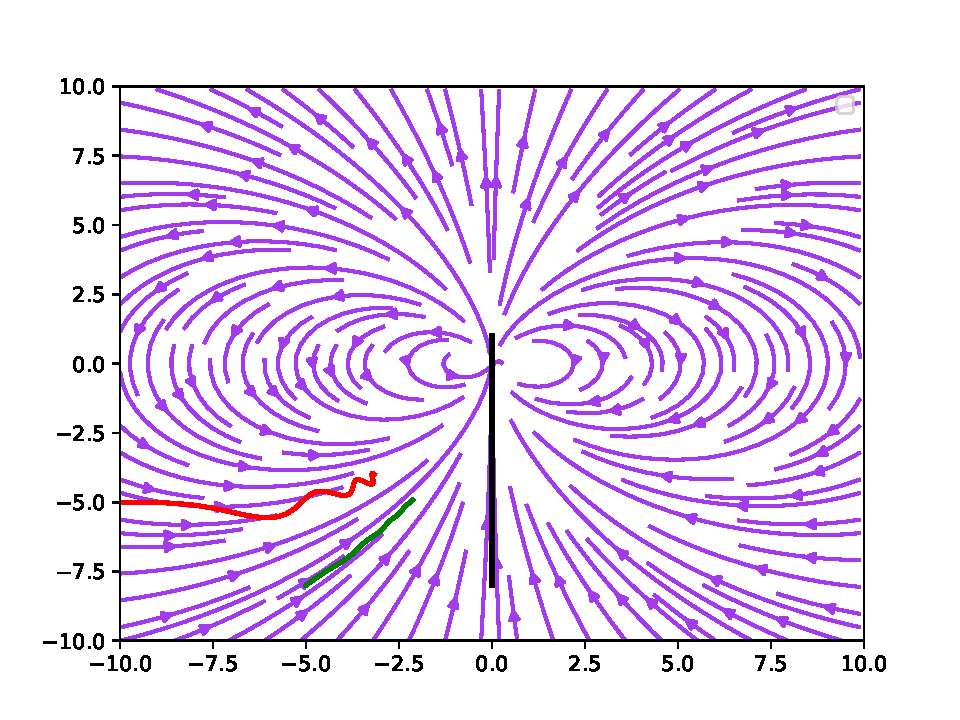
\includegraphics[width=0.8\linewidth]{dipole1.pdf}


\end{center}


\end{document}
